\section{Reinforcement Learning: Q-Learning}

\subsection {``Traditional" Q-Learning} 

After running Q-learning using the parameters provided in the notebook, use the code provided to plot the \textbf{Average Reward, Success Rate, and Car Final Position vs Episodes}. Also give an image of your car reaching the flag in the final episode.
 

% avg reward
 \begin{figure}[H]
   \centering
     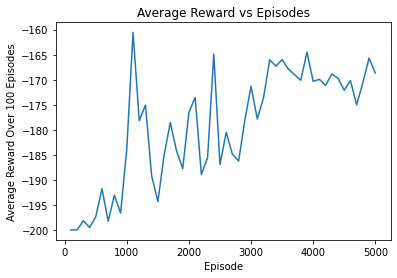
\includegraphics[scale=0.7]
     {templates/avg_reward1}
\end{figure}

% success rate
 \begin{figure}[H]
   \centering
     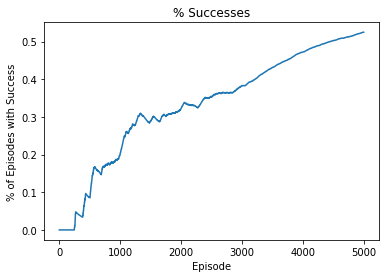
\includegraphics[scale=0.7]
     {templates/success1}
 \end{figure}

% car final position
 \begin{figure}[H]
   \centering
     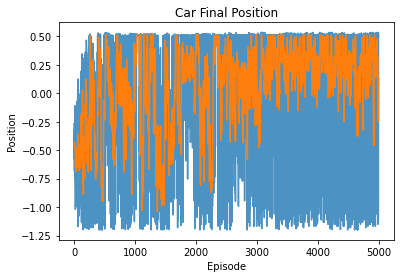
\includegraphics[scale=0.7]
     {templates/position1}
 \end{figure}

% car success image
 \begin{figure}[H]
   \centering
     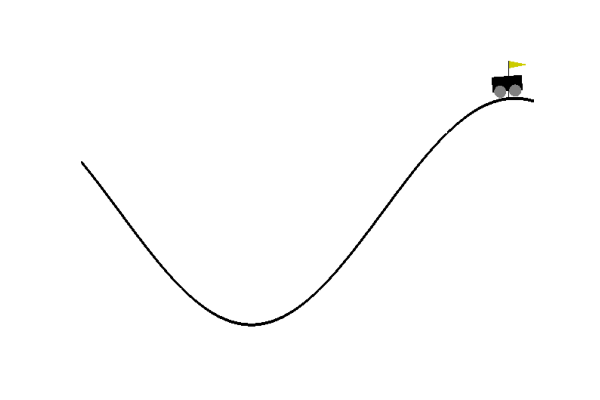
\includegraphics[scale=0.7]
     {templates/car1}
 \end{figure}

\subsection{Deep Q-Learning}

After running deep Q-learning using the parameters provided in the notebook, plot the \textbf{Success Rate, and Car Final Position vs Episodes}.

% success rate, deep
 \begin{figure}[H]
   \centering
     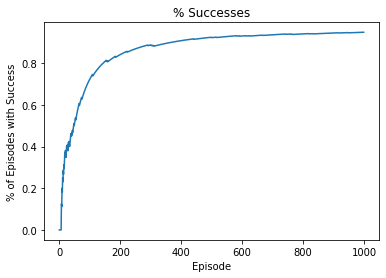
\includegraphics[scale=0.7]
     {templates/success2}
 \end{figure}

% car position, deep 
 \begin{figure}[H]
   \centering
     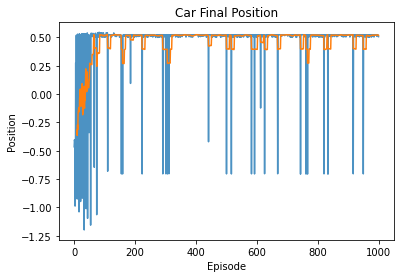
\includegraphics[scale=0.7]
     {templates/position2}
 \end{figure}

 \begin{figure}[H]
   \centering
     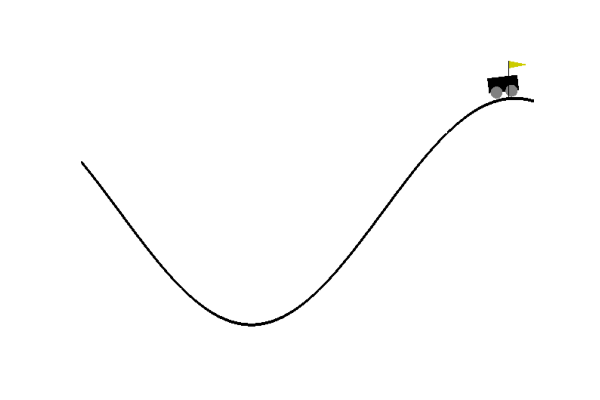
\includegraphics[scale=0.7]
     {templates/car2}
 \end{figure}

\subsection{Questions}
\begin{enumerate}
    \item As part of the Deep QLearning implementation, you implemented a $\mathsf{reward\_shaping}$ function to aid in the learning process. Compare this to the original reward structure in part 2.1 -- why do you think this modification of the reward is helpful?
    \newline
	Description of the reward shaping function: the reward is always 0.5 + the position of the car in the next state, and if the position of the car in the next state is greater than 05, add +1 on top of the computed reward. The original reward structure in 2.1 is un-shaped.
	\newline
	\newline
	In general, Reward shaping augments the natural reward signal in order to provide more frequent feedback on appropriate behaviors during the learning process. This modification of the reward is helpful because it gives the model more feedback during the training process which guides it towards successful outcomes earlier.

    \item Compare the \textbf{Success Rate} and \textbf{Car Final Position} plots between your two implementations. Which algorithm is learning a successful policy more quickly? Briefly comment on potential reasons for any differences in performance.
    \newline\newline
    Differences between the Deep Q-Learning and Standard Q-Learning models: 
    \begin{enumerate}
    \item Car reaches the final position (0.5) within 1000 iterations in the Deep Q-Learning model, whereas the standard Q-Learning model takes 5000 iterations.
    \item Success rate of the Deep Q-Learning model approaches 0.8 as an asymptote within the first 200 episodes, and then steadily makes progress towards a $100\%$ success rate.
    \item The Standard Q-Learning model follows a more linear trajectory in its success rate, and is only able to achieve a $50\%$ success rate at the end of 5000 iterations.
    \end{enumerate}
    
    Based on the above observations, we can conclude that the Deep Q-Learning model learns a successful policy quicker. The potential reasons for these performance differences include: (a) presence of a reward shaping function which provides the model with more feedback during the training process; (b) increased model complexity to better capture the complexity of the optimal policy.
    
\end{enumerate}
